\chapter{上下文敏感对话模型}
本章节介绍本文设计的使用TextCNN和BiLSTM构建分层的上下文敏感对话模型{\dm},旨在分别从句子级别和对话级别对对话文本进行语义表示。首先,通过对聊天消息进行解耦来获取独立解耦对话,然后以对话作为输入文本构建一个分层的上下文敏感对话模型,上下文敏感对话模型{\dm}使用基于TextCNN\cite{kim2014convolutional}对句子进行向量化表示,接下来这些句子向量作为输入,并以对话中对应序列通过BiLSTM\cite{graves2013speech}结构进行编码并获得对话的语义表示。


\section{聊天信息中的对话解耦}
在线聊天是开发者社区之间的一种同步文本通信方式,当一组人在公共的聊天平台进行通信时,聊天中的消息形成流式信息,往往会有很多的对话同时出现,并且经常出现耦合的情况,例如单个会话会与其他会话交织在一起。并且如同 Internet Relay Chat(IRC)、Google Hangout、网站评论等聊天平台不能显式地表明对话的结构,所以无法从中获取独立的会话信息。

将聊天消息划分为一组不同的对话是任何上层对话分析的基本前提,对话解耦就是从一个单一的流信息中识别独立对话的一个任务。
% 目前,关于对话解耦做出重要贡献的是一系列在IRC上标注的数据和训练的模型。Adams和 Martell等人\cite{adams2008topic}研究了对话解耦和话题识别,但是没有公开数据集。Riou等人\cite{riou2015using}在IRC的\#Ubuntu-fr Channel标注对话以及句子关系。Lowe等人\cite{lasecki2013conversations}启发式地从\#Ubuntu Channel进行对话抽取。他们的工作提供了930,000个解耦的对话,为其他对话解耦工作提供了数据基础。Elsner和Charniak等人\cite{elsner2008you}探索了使用信息对特征集和线性分类器,结合局部和全局的推断方法。Jiang等人\cite{jiang2018learning}使用了神经网络的方法,效果达到了提升。
JK Kummerfeld等人\cite{kummerfeld2018large}手工标注了一个大小为77,563条的解耦对话,对于对话定义了一个回复关系图模型,数据集包含内部的对话结构。如图\ref{fig:example-conversation}所示的两个耦合的对话和一个标注的图结构数据是标注数据集的一个样例,其中不同颜色的连线表示图连接。这个例子包括一个当多个人独立的尝试帮助BurgerMann时收到的多个回应的信息,并且在最后消息中BurgerMann回复多个信息。另外,也可以看到delire和Seveas两个用户同时参与两个交谈中。
\begin{figure}[htb]
    \centering
    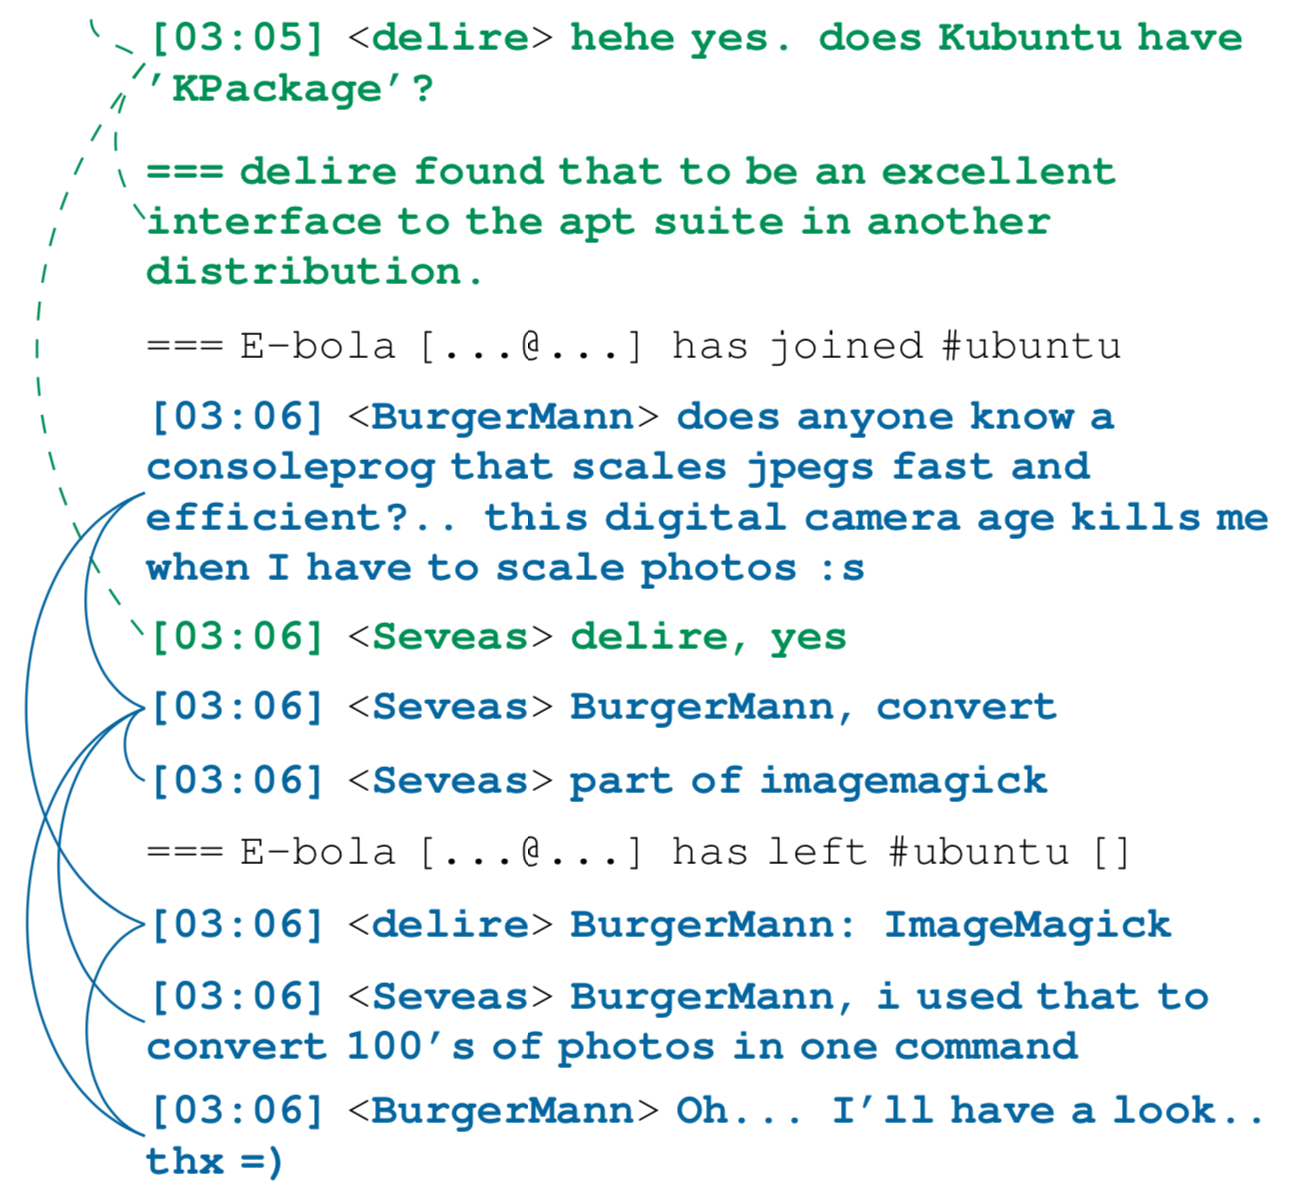
\includegraphics[width=0.4\textwidth]{Img/example-conversation.png}
    \bicaption{Ubuntu的例子。曲线是回复图结构的标注,其中蓝实线和绿虚线分别代表两个对话}{\#Ubuntu log sample. Curved lines are graph annotations of reply structure, which define two conversations shown with blue solid edges and green dashed edges}
    \label{fig:example-conversation}
\end{figure}
作者设计了一个具有2层、512维隐藏层和sigmod非线性激活函数的浅层前馈神经网络,并手工设计了77个特征,其中每个元素都是从原始对话文本中提取的数字类别特征,其中包括当前用户发布的先前聊天消息的时间间隔、聊天内容中是否有目标用户、两个聊天文本是否包含相同的单词等。该模型可以达到74.9%的精度和79.7%的召回率,具有相对较好的效果。

由于JK Kummerfeld等人提出的对话解耦模型为当前效果最好的对话解耦模型,本文选用其研究工作中的模型结构和标注数据对原对话文本进行会话解耦。

\section{上下文敏感对话模型结构设计}
本文设计了一个分层的上下文敏感对话模型{\dm},该模型可以捕获对话中每个句子的语义以及对话整体上下文信息。如图\ref{fig:model}所示,上下文敏感对话模型由四层组成:输入层,句子表示层,对话表示层和输出层。
\begin{figure}[htbp]
    \centering
    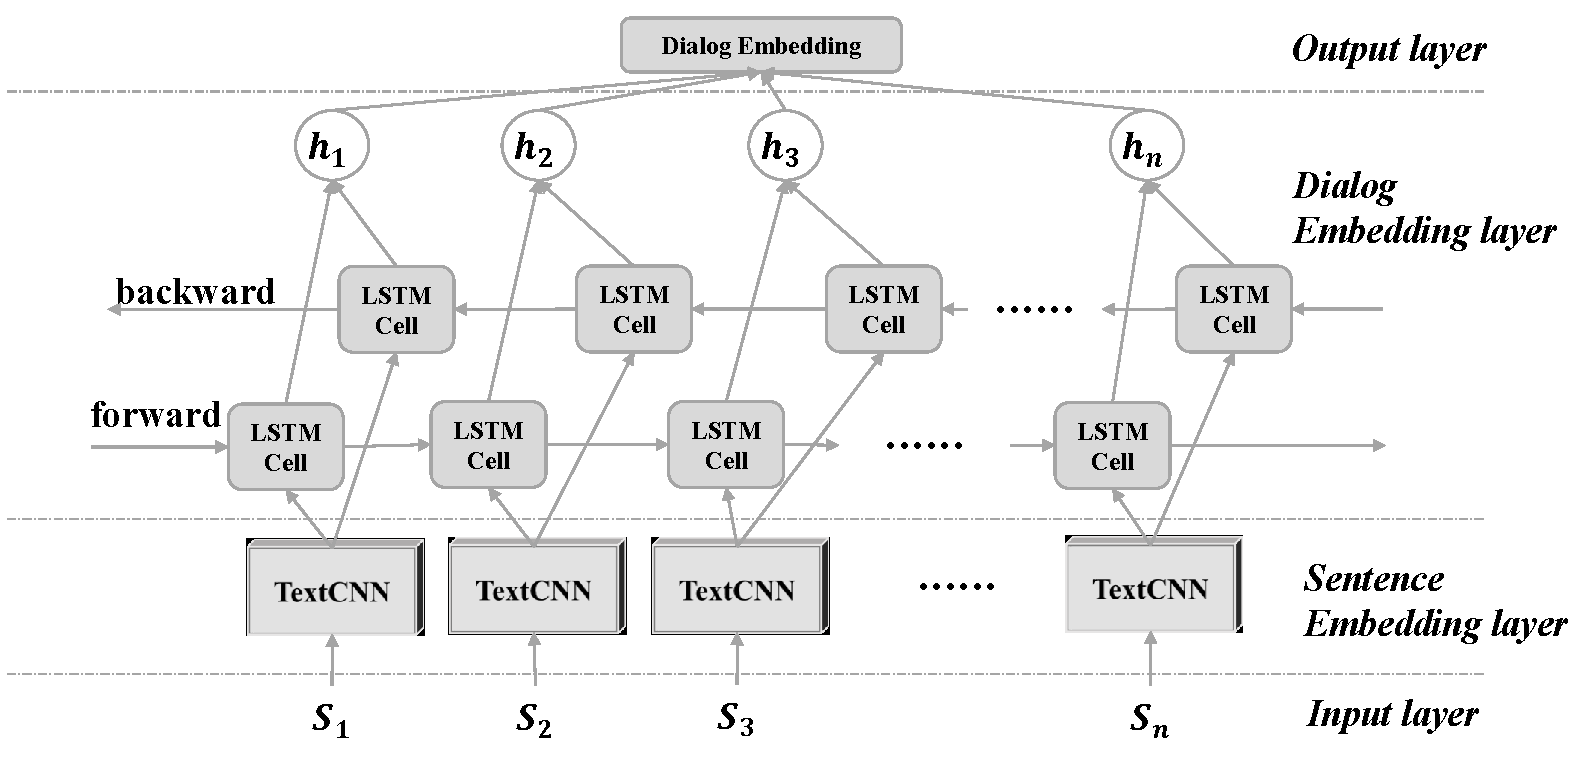
\includegraphics[width=\textwidth]{Img/dialog-model.pdf}
    \bicaption{分层的上下文敏感对话模型{\dm}}{Hierarchical Context-aware Dialog Model {\dm}}
    \label{fig:model}
\end{figure}


% \subsection{BiLSTM}


\subsection{输入层设计}
本文首先将句子分词作为基本元素,然后将词转换为对应的词向量作为模型输入。为了获得更好的效果,本文利用预先在Wikipedia和Gigword语料库上的60亿个单词上经过训练的50维Glove单词向量\cite{pennington2014glove}作为相应单词的初始向量。
% 近来许多研究工作成功地通过学习词的向量空间表示如Word2Vec\cite{mikolov2013distributed}等来细粒度地获取语法和语义信息。这些向量可以被应用在各种任务上,如信息检索、文本分类、自动问答和命名实体识别等。词向量方法使用词对之间的距离或者角度作为评估词表示质量的主要方法。比如:“国王之于王后相当于男人之于女人”,其应该在向量空间表示为“国王-王后=男人-女人”。当前,主要有两种方式进行词向量学习:1)全局矩阵分解方法,如隐式语义分解(LSA)\cite{deerwester1990indexing}等,其使用矩阵的低秩近似将大矩阵进行分解,从而获取语料的统计信息。但是其问题在于高频词将会严重地影响相似度,然而它们是有很少的语义关联的;2)局部上下文窗口方法,如Skip-gram和CBOW方法\cite{mikolov2013distributed},但是其方法局限于只利用了窗口词,没有利用语料巨大的词共现信息。
GloVe是一个无监督的获取词向量的算法,通过在聚集的全局词共现矩阵上进行训练,既使用了语料库的全局统计特征,也使用了局部的上下文特征,其结果显示了在词向量空间的线性特征。GloVe学习词向量的目标是学习词的共现概率比,如词$k$“固体”和词$i$“冰”共现的概率要比和词$j$“蒸汽”共现的概率大,则希望$\frac{P_{ik}}{P_{jk}}$尽可能大,其中$P_{ij}$是词$W_i$出现在词$W_j$上下文的概率。作者据此建立词向量模型:
$$F(w_i, w_j, w_k) = \frac{P_{ik}}{P_{jk}}$$
其中$w_i,w_j,w_k$分别为词$W_i,W_j,W_j$的词向量。为了保持词向量在线性空间的相似性,对模型进一步改进为:
$$exp(w_i^Tw_k-w_j^Tw_k)=\frac{P_{ik}}{P_{jk}}$$
为避免对称性带来的顺序不敏感性,对模型加入偏置项:
$$\log X_{ik}=w_{ik}+b_i+b_k$$
其中$X_{ik}$代表词$W_k$出现在词$W_i$上下文的次数。考虑到词共现的次数越多,这两个词对目标函数影响越大,因此根据词共现次数设计权重对目标函数进行加权:
$$J=\sum_{ik}X_{ik}(w_i^Tw_k+b_i+b_k-\log X_{ik})^2$$
GloVe模型产出了在线性词向量空间上有意义的结果,并达到了超越其他现有模型的效果,尤其在单词相似性比较任务上的表现非常出色。

此外,受先前工作的启发\cite{Sorbo2016Development} \cite{shi2017understanding},注意到需求文本中显式地存在词性(part-of-speech)模式或模板。直观上,pos-tag可以通过引入显式词汇信息来帮助语义理解。因此,本文将pos-tag信息添加到单词表示中以增强其信息表达。具体来说,每种类型的pos-tag都将初始化为具有均匀分布的随机向量,并在训练过程中进行优化。因此,每个单词可以表示为$w_i=[we_i\oplus pos_i]$,其中$we_i$表示相应的单词向量表示,而$pos_i$表示该单词的pos-tag的向量表示。


\subsection{句子表示层设计}
将原始句子转换为单词向量和pos-tag向量拼接的矩阵后,需要通过词信息来建模句子的表示。

在句子表示层中,本文使用TextCNN\cite{kim2014convolutional}来表示句子,因为它使用简洁的网络结构和少量参数,因此在学习不充足的标记数据上具有优势。
TextCNN是用于句子建模的经典方法,它使用浅层卷积神经网络(CNN)\cite{krizhevsky2012imagenet}对句子表示进行建模。CNN是一种已广泛用于计算机视觉的深度学习模型。它使用几个卷积核捕获局部信息,然后使用这些局部信息生成全局表示。类似地,在自然语言处理(NLP)中,CNN可以聚合n元语法信息,并建模句子表示形式。TextCNN将预训练或随机生成的单词嵌入作为输入,其输出的维数取决于卷积核的数量和大小。长度为$n$的句子可以表示为形状为$n\times d$的矩阵,其中$d$是单词嵌入的维数。每个内核为 $w \in \mathbb{R}^{kd}$ ,其中$k$是卷积内核的大小,应用于$k$个单词的窗口,然后映射到一个新的一维向量中。令$X_{i:i+k}$表示原始句子中的\textit{k}-gram单词串,然后对其进行卷积运算。卷积层的输出可以表示为$o_i=f(w\cdot X_{i:i+k} + b)$ ,其中$b$是偏置项,$f$是激活函数。给定一个句子的长度l和卷积核大小$k$,于是可以获得大小为$l-k+1$的句子的表示形式。卷积层后面是最大池化层,它可以捕获具有最大值的关键信息。
为了获得由不同尺度的局部信息组合而成的更充分的语义信息,可以将具有不同大小的多个卷积核应用于该句子。 因此,对于一个给定$n \times m$积核的句子,其中$n$是不同大小的核数,而$m$是每种大小的数量,可以得到大小为 $n\times m$的句子表示形式,其将不同尺度的局部信息转化为句子的整体表示。

如图\ref{fig:textcnn}所示为TextCNN应用在句子分类上的模型结构图,其中不同颜色的矩阵为不同大小的二维卷积核,输出为二维向量用于句子分类。本文中分别使用2,3,4,5大小的不同尺度卷积核对句子特征进行建模表示。
\begin{figure}[htb]
    \centering
    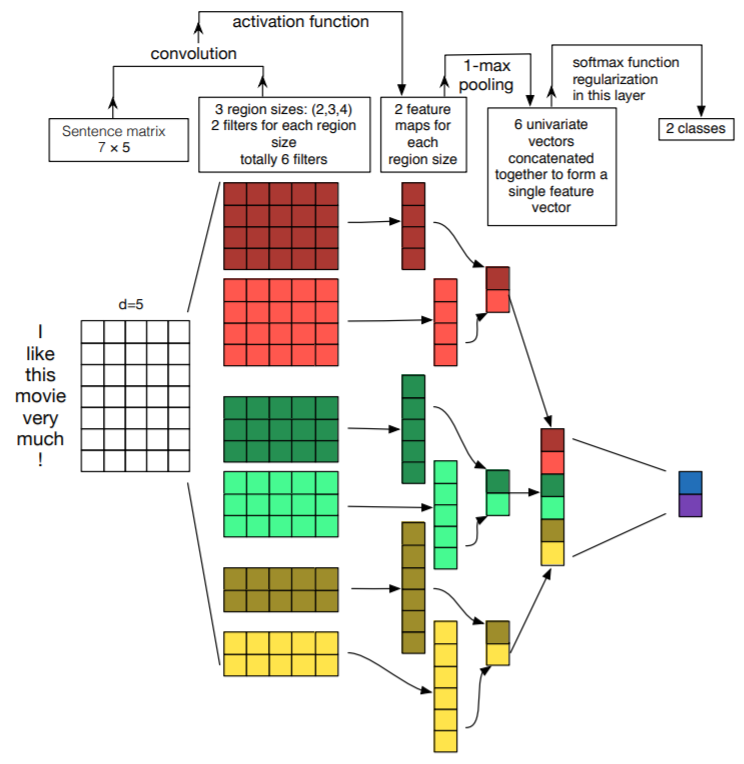
\includegraphics[width=0.6\textwidth]{Img/textcnn.png}
    \bicaption{一个用于句子分类的CNN结构表示}{Illustration of a CNN architecture for sentence classification}
    \label{fig:textcnn}
\end{figure}

\subsection{对话表示层设计}
分析来自聊天消息的对话是一项上层的文本挖掘任务,因为当理解一个句子时,它需要考虑对话范围内的上下文信息,因此针对对话级别的表示建模中,本文利用双向长期短期记忆网络(BiLSTM\cite{graves2013speech}),将对话的句子视为顺序序列,以捕获上下文信息,其中句子的表示由TextCNN表示。BiLSTM为序列学习任务编码双向信息,其堆叠两个方向相反的标准LSTM层,以分别学习句子的单向表示。然后,它将前向和后向表示形式组合为双向嵌入。LSTM是基于Hochreiter等人\cite{hochreiter1997long}提出的基于门机制的优化的递归神经网络(RNN)结构。LSTM利用门机制来提取关键信息,并将其传递给后面的长序列。LSTM单元由输入门,忘记门,单元状态和输出门组成。如图\ref{fig:lstm}(\subref{fig:lstm})所示为LSTM单元的模型结构。
\begin{figure}[htb]
    \centering
    \begin{subfigure}[b]{0.45\textwidth}
      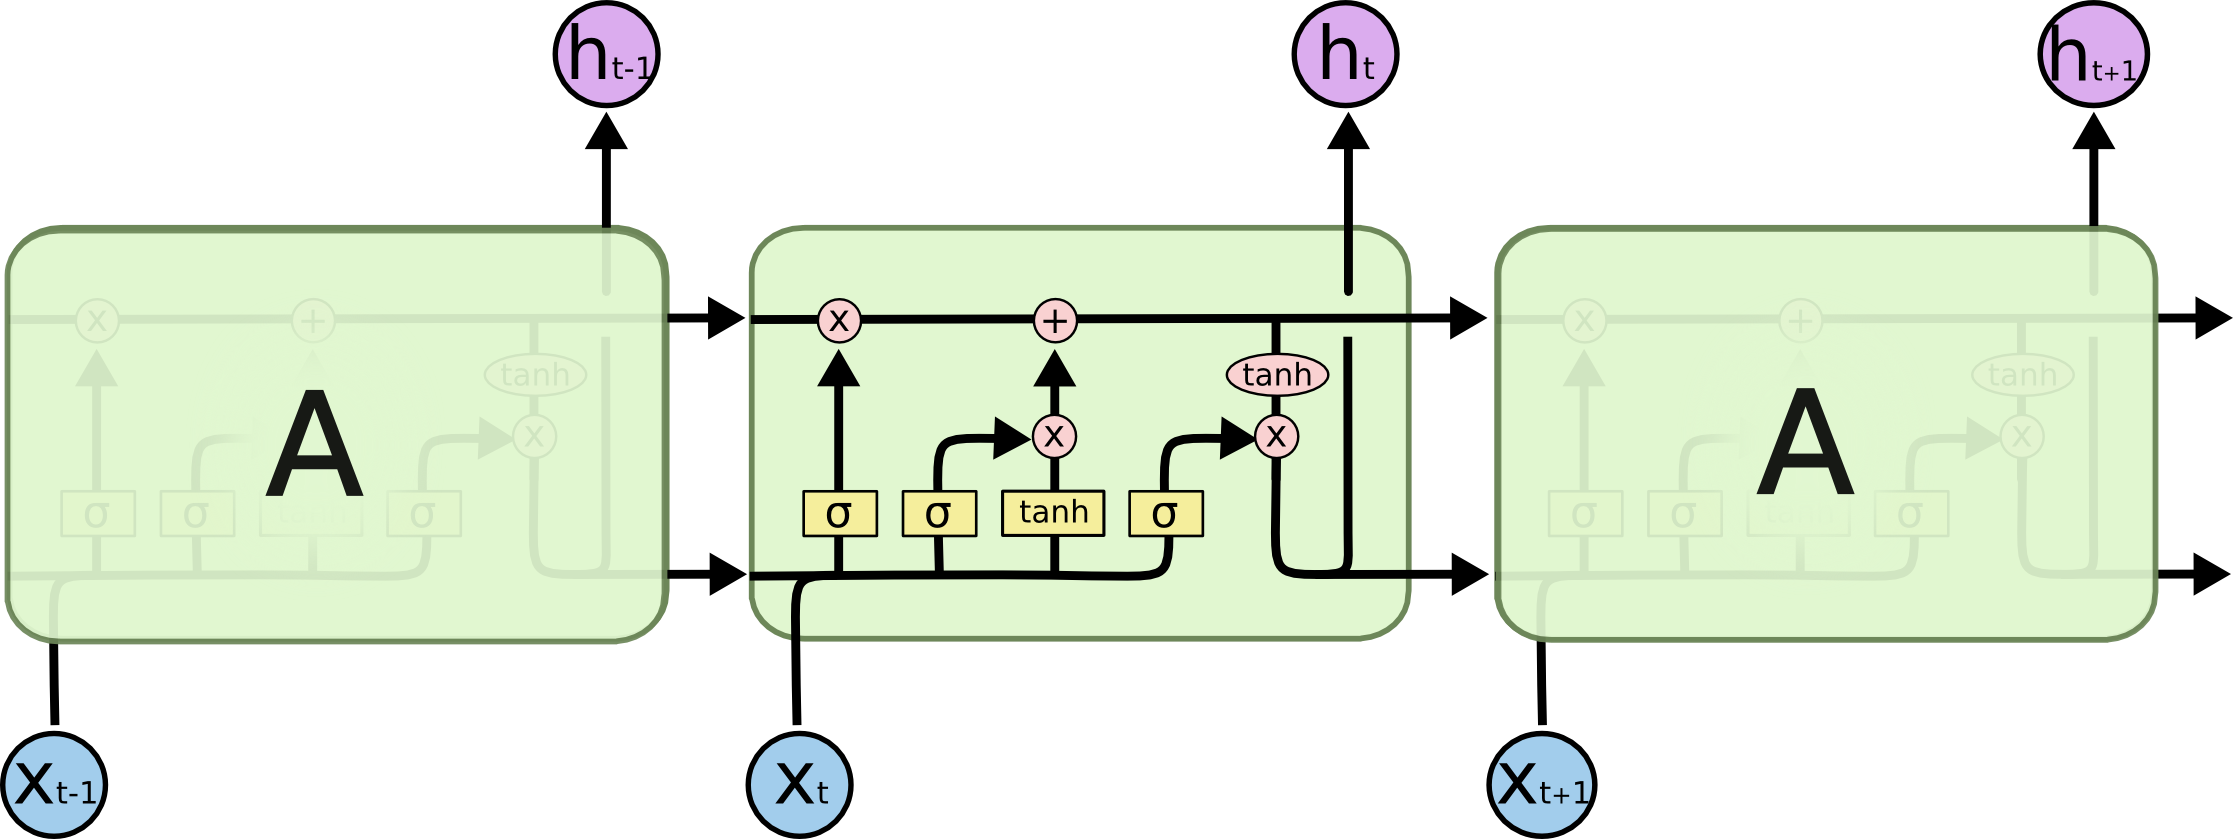
\includegraphics[width=\textwidth]{Img/lstm.png}
      \caption{}
      \label{fig:lstm}
    \end{subfigure}%
    ~% add desired spacing
    \begin{subfigure}[b]{0.45\textwidth}
      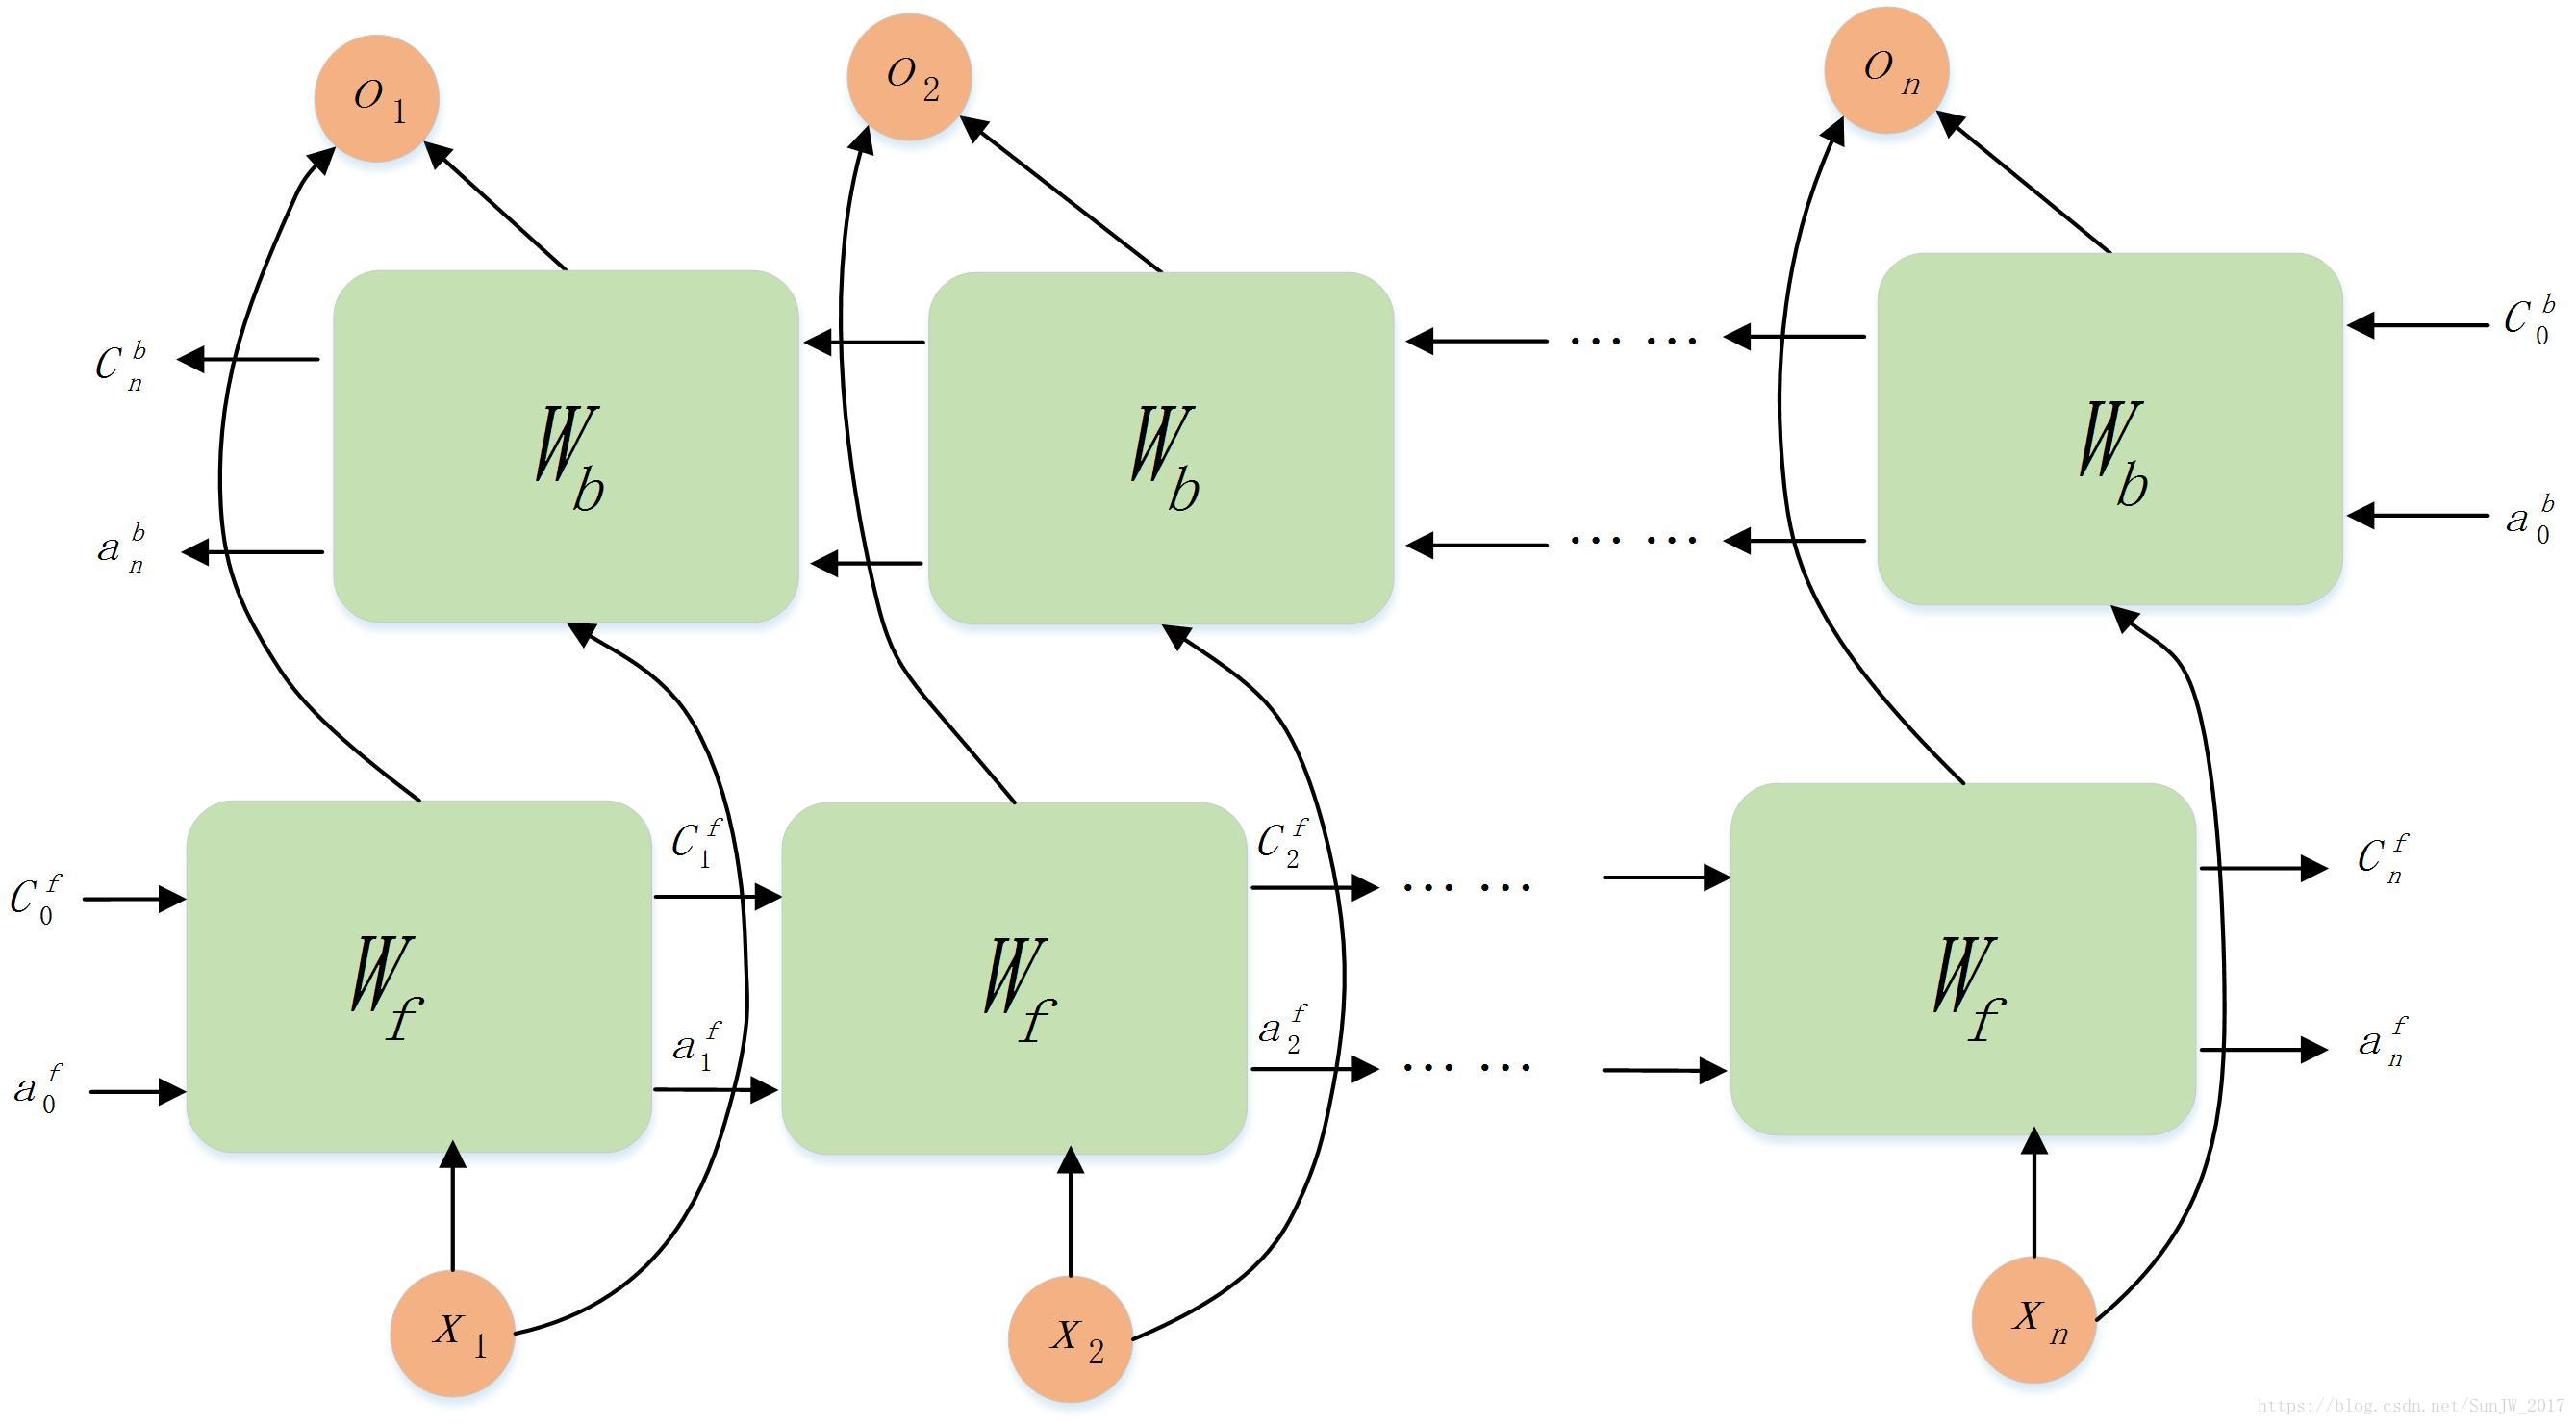
\includegraphics[width=\textwidth]{Img/bilstm.jpg}
      \caption{}
      \label{fig:bilstm}
    \end{subfigure}
    \bicaption{LSTM和BiLSTM结构。(a) 为LSTM结构,(b) 为BiLSTM,其使用两个LSTM}{The architectures of LSTM and BiLSTM. (a) LSTM structure, (b) BiLSTM structure, which uses two LSTM}
    \label{fig:lstm}
\end{figure}

% \begin{figure}[htb]
%     \centering
%     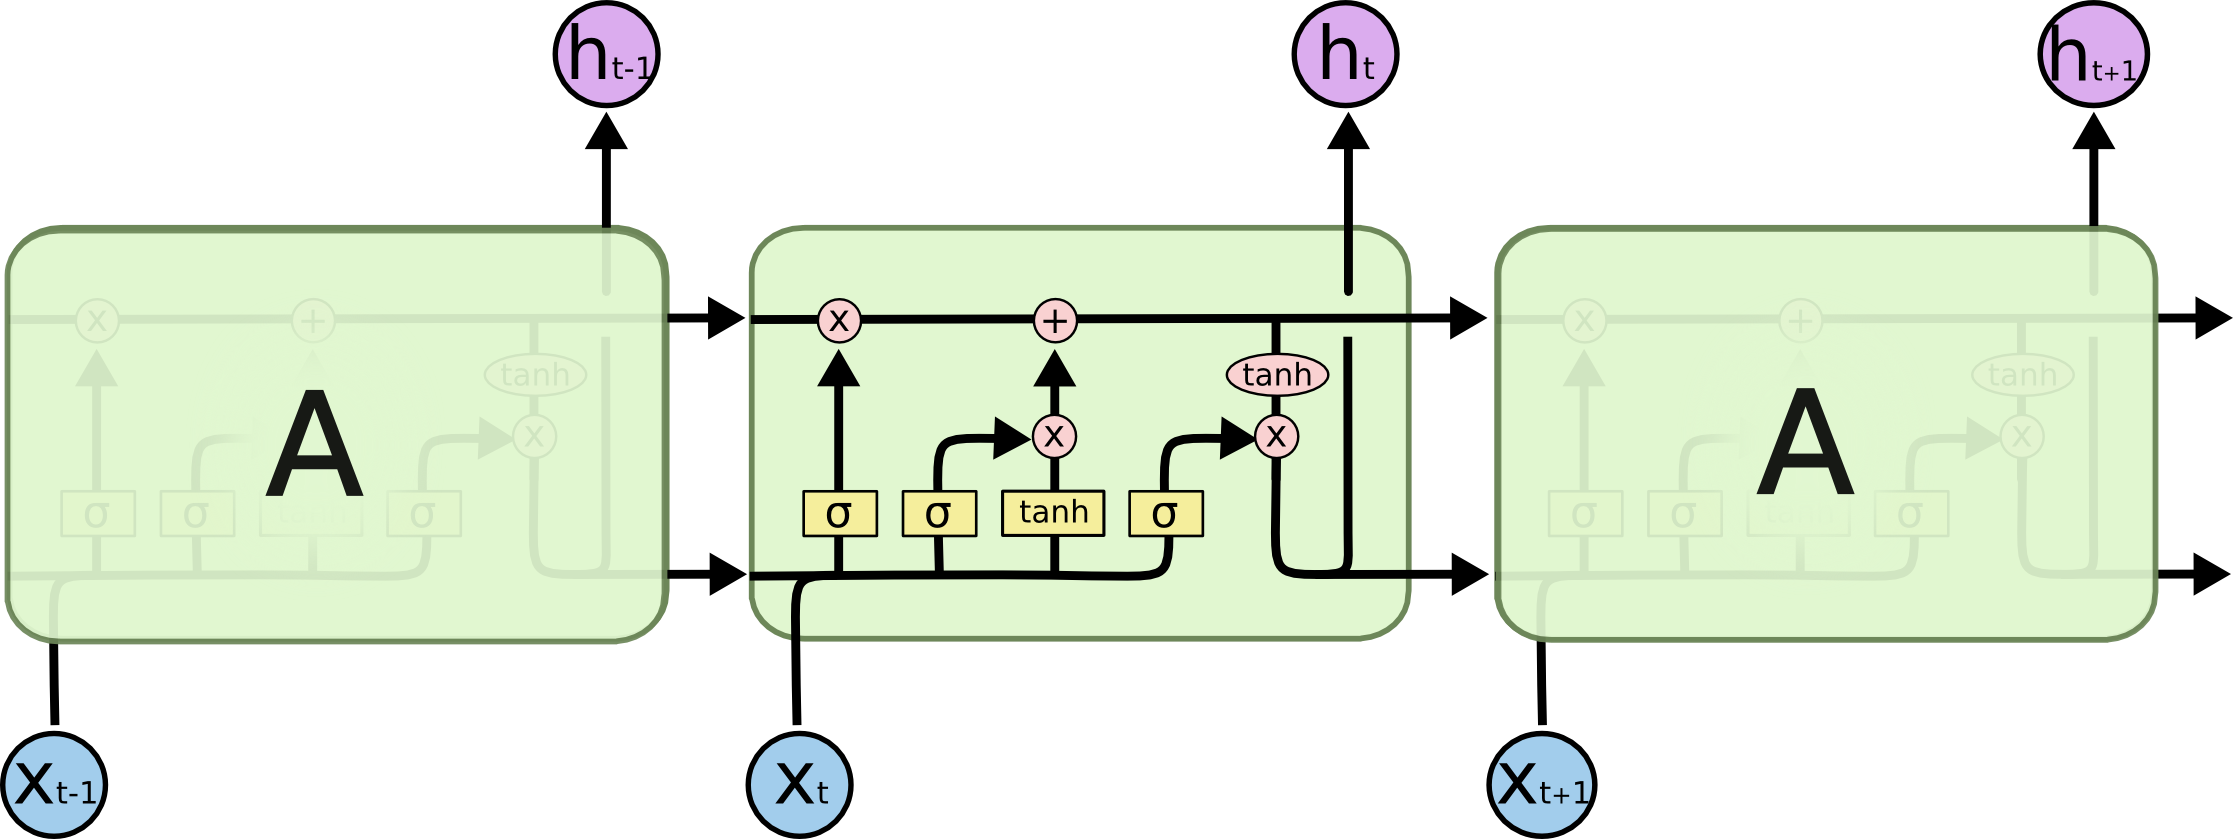
\includegraphics[width=0.6\textwidth]{Img/lstm.png}
%     \bicaption{一个LSTM单元的结构表示}{Illustration of an LSTM cell architecture}
%     \label{fig:lstm}
% \end{figure}
其中,LSTM单元门的输出可以表示如下:
$$\begin{aligned}\left[\begin{array}{c}{{\mathbf{i}_{t}} \\ {\mathbf{f}_{t}} \\ \tilde{\mathrm{c}}_{t}} \\ {\mathbf{o}_{t}}\end{array}\right] &=\left[\begin{array}{c}{\sigma} \\ {\sigma} \\ {tanh} \\ {\sigma}\end{array}\right] \left( \mathbf{W} \left[\begin{array}{c}{\mathbf{x}_{t}} \\ {\mathbf{h}_{t-1}}\end{array}\right] +\mathbf{b} \right)  \tag{1} \\ \mathbf{c}_{t} &=\tilde{\mathbf{c}}_{t} \odot \mathbf{i}_{t}+\mathbf{c}_{t-1} \odot \mathbf{f}_{t} \tag{2} \\ \mathbf{h}_{t} &=\mathbf{o}_{t} \odot \tanh \left(\mathbf{c}_{t}\right) \tag{3} \end{aligned}$$
其中$\mathbf{x}_{t}$ 是在这个输入句子中的第$i^{th}$个token,$\mathbf{W}$是LSTM单元的权重矩阵,$\mathbf{b}$是偏置项,$\mathbf{\sigma}$是sigmod激活函数,$\mathbf{tanh}$是双曲正切函数,$\odot$是element-wise的乘法。
因此,BiLSTM最终可表示为 $h=[\overrightarrow{h}\oplus \overleftarrow{h}]$,其中 $ \overleftarrow{h}$ 和  $ \overleftarrow{h}$分别表示两层LSTM的输出, $\oplus$ 表示连接运算。
如图\ref{fig:lstm}(\subref{fig:bilstm})所示为BiLSTM的结构示意图。
% \begin{figure}[htb]
%     \centering
%     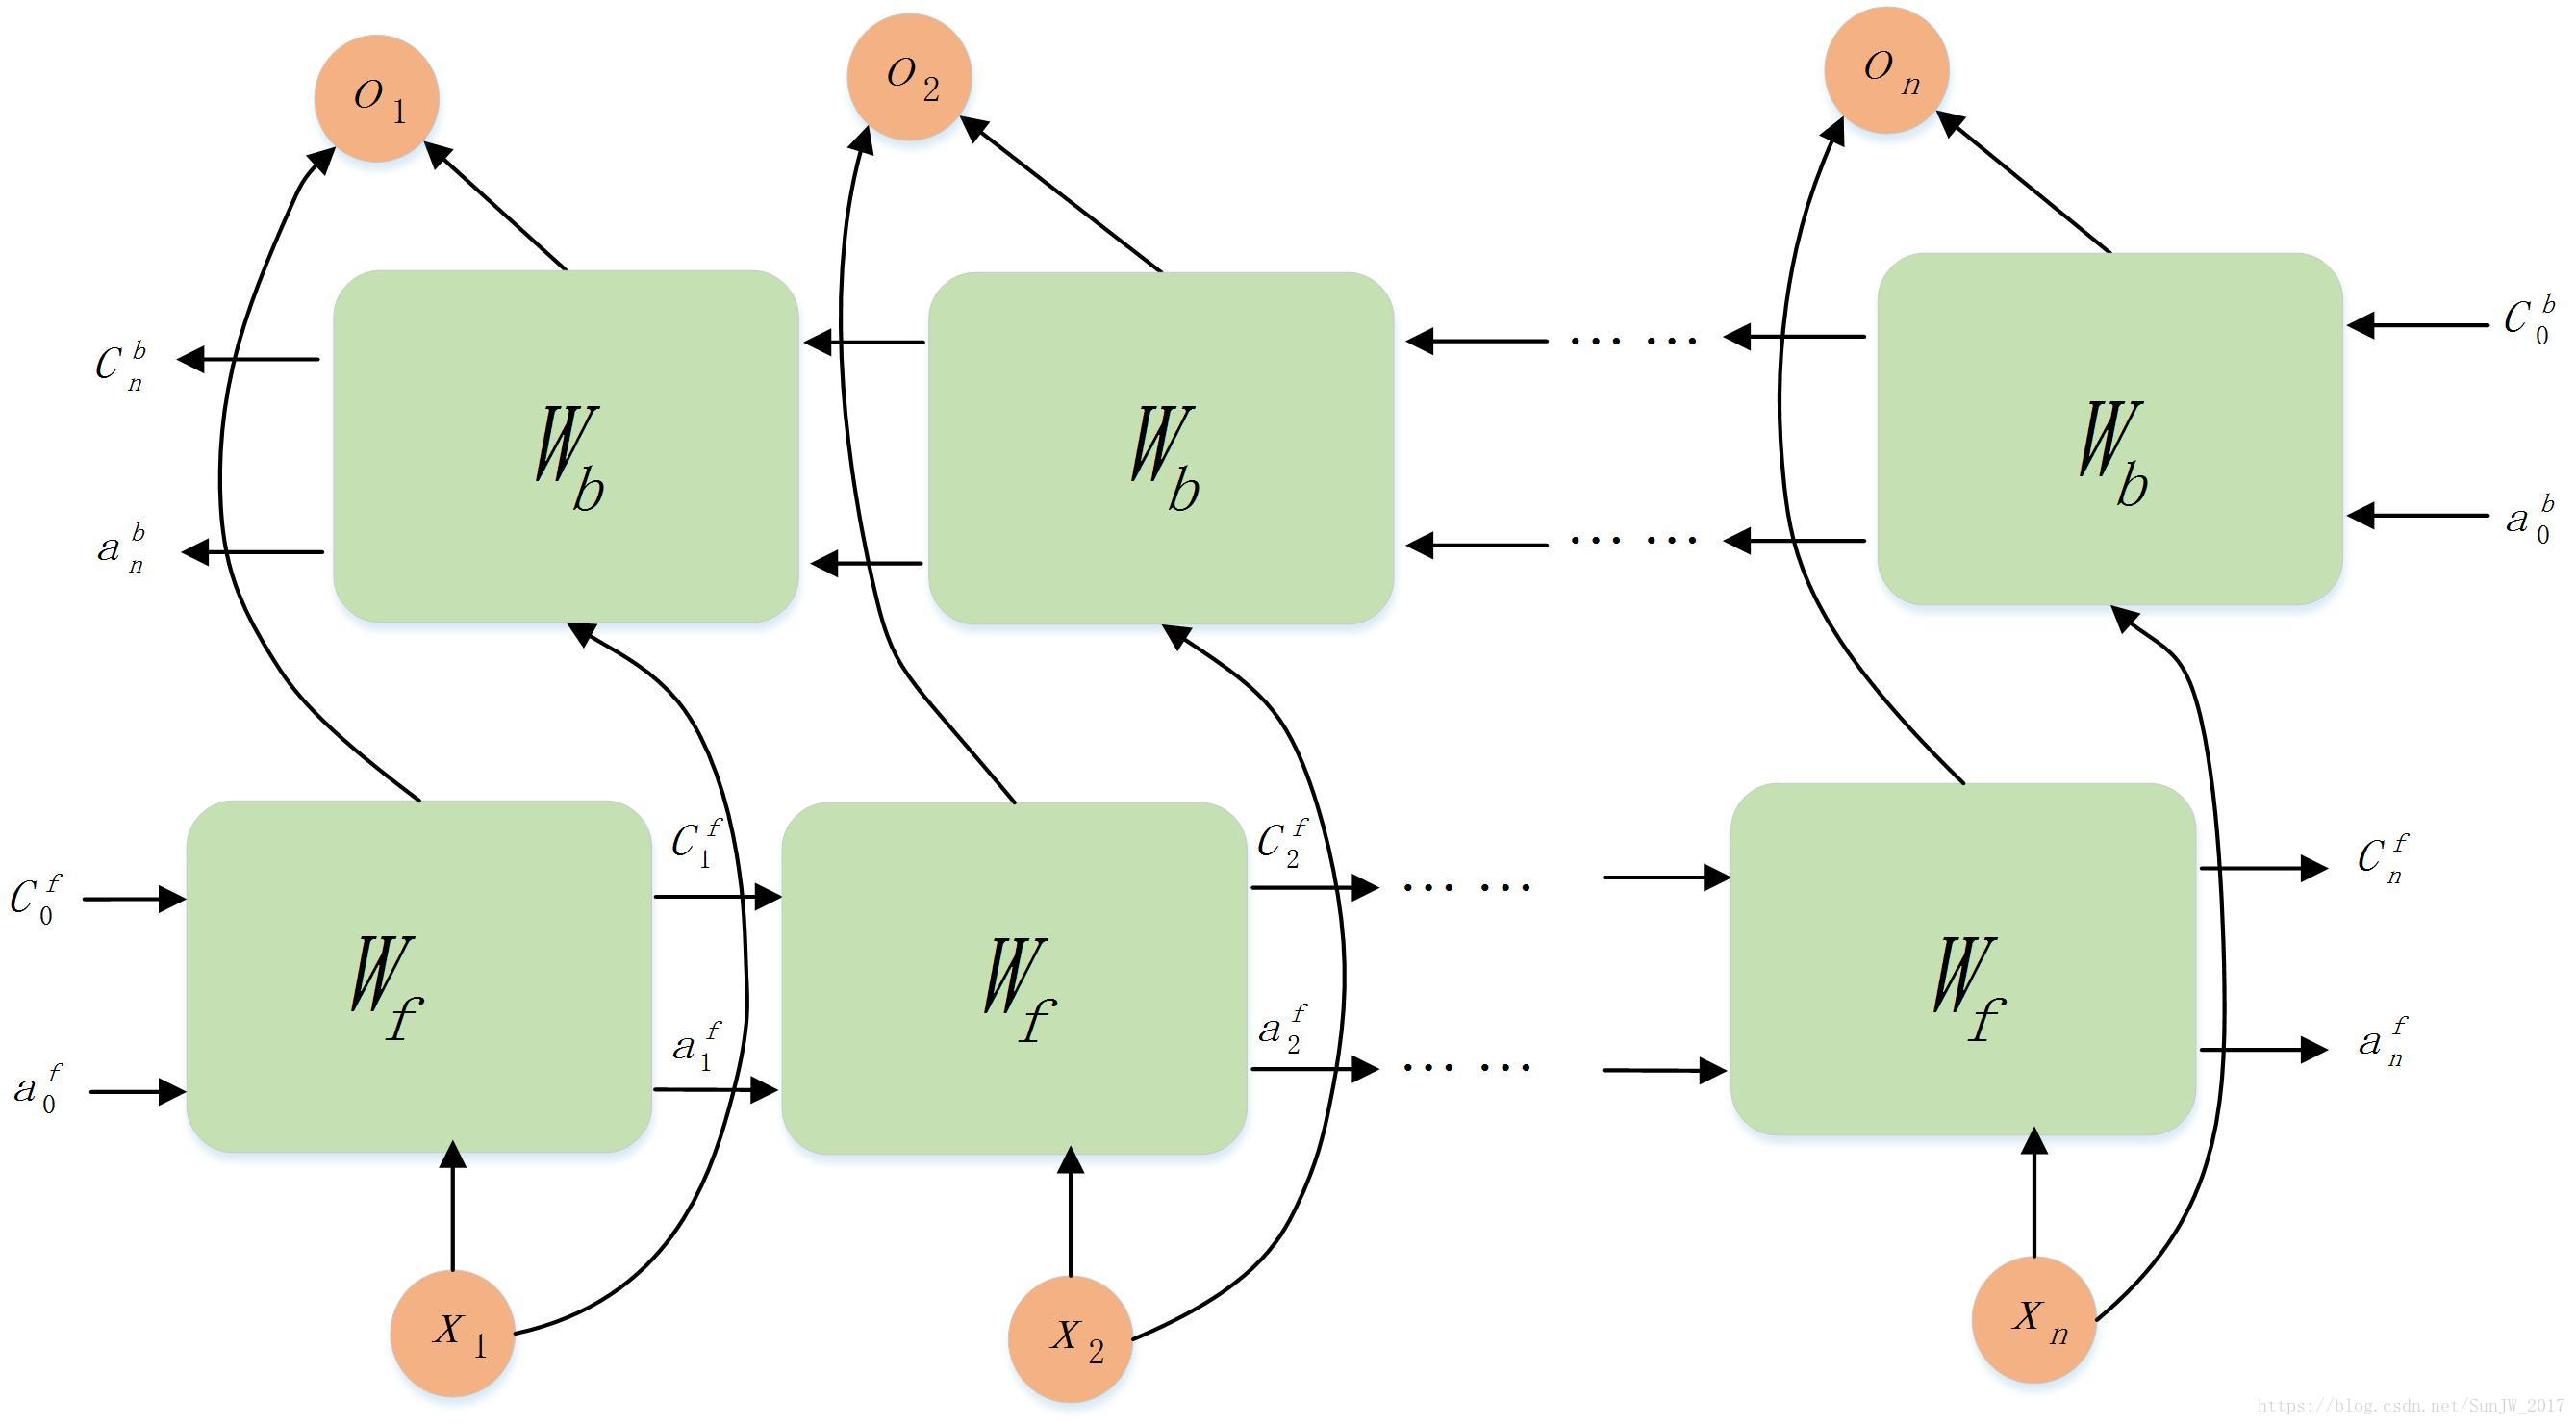
\includegraphics[width=0.4\textwidth]{Img/bilstm.jpg}
%     \bicaption{BiLSTM的结构表示}{Illustration of BiLSTM architecture}
%     \label{fig:bilstm}
% \end{figure}
本文使用一系列句子向量来表示对话,当把句子根据对话中的顺序输入BiLSTM编码器时,每个向量表达的句子都被当作基本单元。在对BiLSTM进行编码之后,可以学习对话的双向上下文信息。

\subsection{输出层设计}
\textbf{输出层:}在输出层中,本文组合由BiLSTM编码的两个方向表示$\overrightarrow{h}$和$\overleftarrow{h}$作为对话的输出向量,其可以表示为$h=[\overrightarrow{h}\oplus \overleftarrow{h}]$。

% \section{上下文敏感对话分类模型设计}
% 本文目的在于对从聊天记录中解耦得到的对话进行分类,并将对话分类为表示需求意图的对话和不是需求意图的对话,从而达到从聊天记录中进行隐藏需求对话识别的目的。为了清楚起见,在下文中,将使用\textit{feature dialog}和\textit{non-feature dialog}来表示需求意图的对话和不是需求意图的对话。

% 对话经过上下文敏感对话模型之后,在输出层可以得到对话对应的向量化表示,该向量化表示可以应用于如线性前馈网络等分类层从而进行文本分类。
% 本文构建了一个上下文敏感对话分类模型plain-{\tool},下文中使用p-{\tool}表示该模型。其模型结构图如图\ref{fig:model-cls}所示,模型是在前文所述的上下文敏感对话模型的基础上添加线性分类层,其可以对需求对话进行分类识别。
% \begin{figure}[htbp]
%     \centering
%     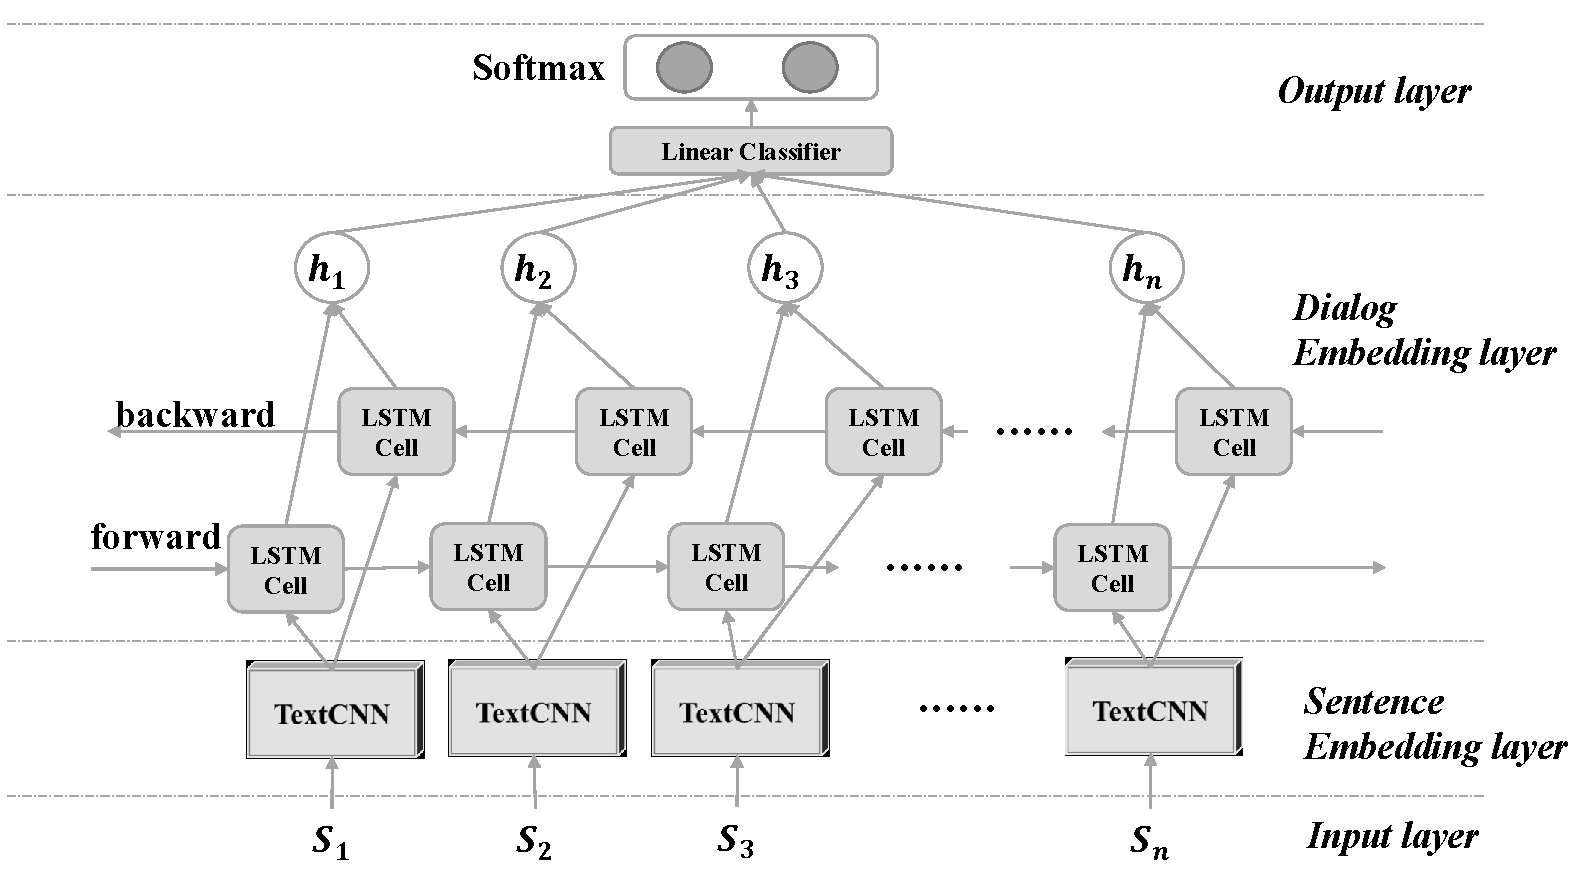
\includegraphics[width=\textwidth]{Img/model_cls.pdf}
%     \bicaption{p-{\tool}上下文敏感对话分类模型}{p-{\tool} Context-aware Dialog Classification Model}
%     \label{fig:model-cls}
% \end{figure}

% 由于每个对话都属于\textit{feature dialog}类或\textit{non-feature dialog}类,因此分类层输出为长度为2的向量$[score_1 , score_2]$  ,代表两个类的分数,其中$score_i \in \mathbb{R}$ 。 接下来对此向量执行softmax,表示为
% $$Softmax(socre_i)=\frac{e^{score_i}}{\sum_{j=1}^2 e^{score_j}}$$ 
% ,可以将 $[score_1 , score_2]$ 归一化为概率$[p ,1-p]$,其中 $p \in [0,1]$。

% \section{上下文敏感对话模型实现}

% 在模型实现部分,p-{\tool}使用AllenNLP\footnote{https://allennlp.org/},一个基于PyTorch\footnote{https://pytorch.org/}构建的开源NLP库来进行实现。

% 在代码实现上下文敏感对话模型结构时,主要继承AllenNLP的\textit{Model}类,其实现了NLP中一些常见的方法,如Vocabulary中word到index的映射、参数初始化、正则项等,这些方法可以为{\tool}的实现减少大量的重复工作。

% 对于训练过程,主要继承了AllenNLP的\textit{Trainer}类,其实现了一些神经网络训练过程中常用的方法,如序列化保存、GPU训练、数据集加载、梯度裁剪、TensorBoard可视化等。训练过程中所需要的参数保存在json文件中,AllenNLP加载json文件并初始化\textit{Trainer}类,然后开始进行训练以及评估测试。

% 对于超参数,本文选用Grid Search\cite{Bergstra2012Random}作为参数选择方法以获得最佳效果。pos-tag向量的维度为50,与单词向量相同。然后,可以使用$s=[w_1,w_2\dots w_n]$ 作为句子的表示形式,其中$w_i=[we_i\oplus pos_i]$。为了获得由不同尺度的局部信息组合而成的更充分的语义信息,本文对句子应用具有不同大小的多个卷积核,其大小分别是2、3、4、5,每类卷积核有25个。BiLSTM的输出维度为300(每个方向是150维)。由于该任务可以视为分类问题,因此本文将交叉熵用作损失函数。

% 此外,为避免过拟合问题,本文以0.1的dropout rate对输入向量进行Dropout \cite{srivastava2014dropout},这意味着将随机屏蔽10%的神经元以减少每次批量训练中需要训练的参数。本文还使用了Early Stopping\cite{prechelt1998early}的策略,如果测试数据集的效果在10个Epoch内未提升,则训练过程将停止。对于神经网络的优化器,由于Adam\cite{kingma2014adam}对梯度的一阶矩估计和二阶矩估计进行综合考虑,并且其具有自适应性能好、参数的更新不受梯度的伸缩变换影响等特点,本文使用Adam优化器对模型参数进行更新优化。

\section{本章小结}

本章介绍了对话解耦这一对流式聊天记录进行对话信息必不可少的步骤,以及本文中使用的对话解耦模型。接下来介绍通过分层的、分别使用TextCNN和BiLSTM对句子和对话级别进行语义表示的上下文敏感对话模型{\dm},该模型可以将对话转换为向量化表示,该向量嵌入了对话的语义信息,并使该对话信息应用到下文中的需求识别任务中。
% 另外,针对上下文敏感对话模型,本章构建了p-{\tool},该模型通过增加线性分类层可以对对话进行分类,从而达到需求识别的目的。最后,介绍了p-{\tool}的模型实现相关细节。
